\section{Training Approach}

\begin{outline}
  Describe the reinforcement learning or supervised learning approach
  used to train the CNN models.
\end{outline}

As in \cite{bratta_contactnet_2024}, the cost maps are normalized to
improve training performance
(\autoref{fig:data-cn-cost-map-normalization}). This approach differs
though because the cost maps are normalized independently for each
leg, rather than across all legs. This is necessary because we are
using a separate model for each leg. This strips the leg priority
information from the data, reducing it to only the best positions for
each leg. The leg priority will be learned by the GaitNet.

\begin{figure}
  \centering
  \begin{minipage}[T]{0.45\textwidth}
    \centering
    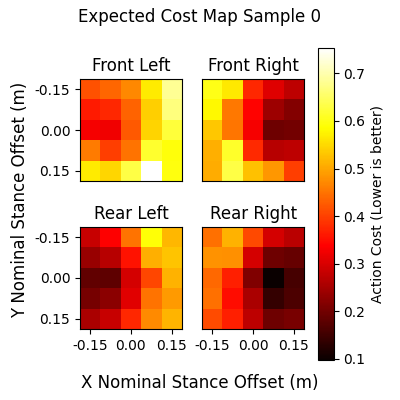
\includegraphics[width=\textwidth]{images/data/cost-map-normalization/un-normalized.png}
  \end{minipage}
  \hfill
  \begin{minipage}[T]{0.45\textwidth}
    \centering
    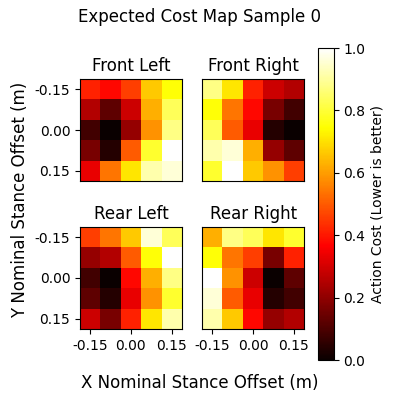
\includegraphics[width=\textwidth]{images/data/cost-map-normalization/normalized.png}
  \end{minipage}
  \hfill

  \caption{Cost map normalization showing un-normalized (left) and
  normalized (right) cost maps.}
  \label{fig:data-cn-cost-map-normalization}
\end{figure}

Below is the equation used as the input to the contact model.

\[
  \mathbf{x} =
  \begin{bmatrix}
    \mathbf p_{b,xy} \\
    \mathbf r_{w,z} \\
    \mathbf v_b \\
    \mathbf \omega_b \\
    \mathbf u
  \end{bmatrix}
\]

where
$\mathbf p_{b,xy}$ is the $x$ and $y$ position all end effectors in
the base frame as a single vector,
$\mathbf r_{w,z}$ is the height of the robot's COM in the world frame.

The model is trained on $y$, the heuristically calculated footstep
cost maps (\autoref{fig:data-footstep-cost-map}).

Here, the inclusion of $\mathbf \omega_b$ differs from
\cite{bratta_contactnet_2024}

The results of this model are very promising, with the model able to
predict footstep cost maps with high accuracy.
\autoref{fig:data-cn-typical-data-comparison}
shows the model output and ground truth for typical data sample.
\autoref{label:data-cn-typical-data-comparison}
shows a particularly challenging data sample, and the model is still
able to identify the best positions for each leg,
particularly the back left leg, which needs to be far from the
nominal position to maintain stability in that state.

\begin{figure}
  \centering
  \begin{minipage}[T]{0.45\textwidth}
    \centering
    \includegraphics[width=\textwidth]{images/data/training/typical-expected.png}
  \end{minipage}
  \hfill
  \begin{minipage}[T]{0.45\textwidth}
    \centering
    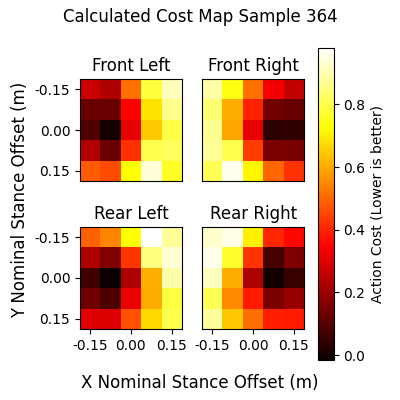
\includegraphics[width=\textwidth]{images/data/training/typical-calculated.png}
  \end{minipage}
  \hfill

  \caption{Typical data samples showing calculated (left) and
  expected (right) quadruped images.}
  \label{fig:data-cn-typical-data-comparison}
\end{figure}

\begin{figure}
  \centering
  \begin{minipage}[T]{0.45\textwidth}
    \centering
    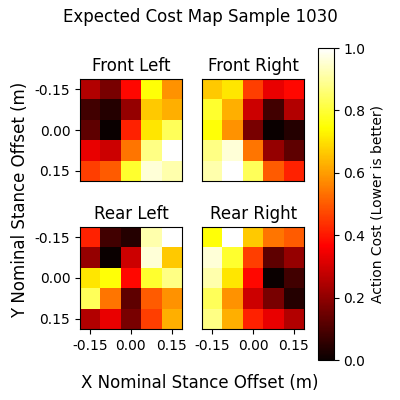
\includegraphics[width=\textwidth]{images/data/training/challenging-expected.png}
  \end{minipage}
  \hfill
  \begin{minipage}[T]{0.45\textwidth}
    \centering
    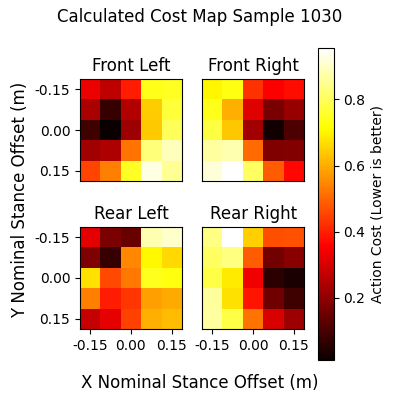
\includegraphics[width=\textwidth]{images/data/training/challenging-calculated.png}
  \end{minipage}
  \hfill

  \caption{Particularly challenging data samples showing calculated (left) and
  expected (right) quadruped images.}
  \label{fig:data-cn-challenging-data-comparison}
\end{figure}
